% \documentclass{article}
\documentclass{book}
% \documentclass{report}
\usepackage{amsmath}
\usepackage{fontspec}
\usepackage{xunicode}
\usepackage{indentfirst}
% add algorithm
\usepackage{algorithm}  
\usepackage{algorithmic}
\usepackage{graphicx}  

%chinese
\usepackage{xeCJK}

% from denny
\usepackage[utf8]{inputenc}
\usepackage{amssymb}
\usepackage{subfig}
\usepackage{bbm}
% for block

\usepackage[dvipsnames,svgnames]{xcolor}
% \usepackage[usenames, dvipsnames]{color}
\definecolor{mypink2}{RGB}{219, 48, 122}
\definecolor{mypink3}{cmyk}{0, 0.7808, 0.4429, 0.1412}

\colorlet{LightRubineRed}{RubineRed!70!}
\colorlet{Mycolor1}{green!10!orange!90!}
\definecolor{Mycolor2}{HTML}{00F9DE}

% \pagecolor{black}
% \color{white}
% alert 
\usepackage{environ}
% \usepackage{xcolor}
\usepackage[tikz]{bclogo,rotating}
\usepackage{tikz}
\usetikzlibrary{calc}
\usepackage{lipsum}
\DeclareGraphicsRule{.mps}{eps}{.mps}{}

\usepackage{stmaryrd}
 
\NewEnviron{myremark}[1]
  {\par\medskip\noindent
  \begin{tikzpicture}
    \node[inner sep=0pt] (box) {\parbox[t]{.99\textwidth}{%
      \begin{minipage}{.3\textwidth}
      \centering\tikz[scale=5]\node[scale=3,rotate=30]{\bclampe};
      \end{minipage}%
      \begin{minipage}{.65\textwidth}
      \textbf{#1}\par\smallskip
      \BODY
      \end{minipage}\hfill}%
    };
    \draw[red!75!black,line width=3pt]
      ( $ (box.north east) + (-5pt,3pt) $ ) -- ( $ (box.north east) + (0,3pt) $ ) -- ( $ (box.south east) + (0,-3pt) $ ) -- + (-5pt,0);
    \draw[red!75!black,line width=3pt]
      ( $ (box.north west) + (5pt,3pt) $ ) -- ( $ (box.north west) + (0,3pt) $ ) -- ( $ (box.south west) + (0,-3pt) $ ) -- + (5pt,0);
  \end{tikzpicture}\par\medskip%
}

\graphicspath{ {pic/} }

%% XeTeX adds code when switching latin (0) or boundary (255) to CJK (1, 2, 3)
\XeTeXinterchartokenstate = 1

%% Fonts for Latin and CJK
\newfontfamily\rmfont{TeX Gyre Pagella}
\newfontfamily\cjkfont{SimSun}

%% Ranges for Latin Font
\XeTeXinterchartoks 1 0 = {\rmfont}
\XeTeXinterchartoks 2 0 = {\rmfont}
\XeTeXinterchartoks 3 0 = {\rmfont}
\XeTeXinterchartoks 255 0 = {\rmfont}

%% Ranges for CJK Font
\XeTeXinterchartoks 0 1 = {\cjkfont}
\XeTeXinterchartoks 0 2 = {\cjkfont}
\XeTeXinterchartoks 0 3 = {\cjkfont}
\XeTeXinterchartoks 255 1 = {\cjkfont}
\XeTeXinterchartoks 255 2 = {\cjkfont}
\XeTeXinterchartoks 255 3 = {\cjkfont}

\XeTeXlinebreaklocale "zh"
\XeTeXlinebreakskip = 0pt plus 1pt

\DeclareMathOperator*{\argmin}{arg\,min}
%%%%%%%%copy from http://www.latextemplates.com/cat/title-pages
\newcommand*{\plogo}{\fbox{$\mathbb{ML}$}} % Generic publisher logo
%----------------------------------------------------------------------------------------
%	TITLE PAGE
%----------------------------------------------------------------------------------------

\newcommand*{\rotrt}[1]{\rotatebox{90}{#1}} % Command to rotate right 90 degrees
\newcommand*{\rotlft}[1]{\rotatebox{-90}{#1}} % Command to rotate left 90 degrees

\newcommand*{\titleBC}{\begingroup % Create the command for including the title page in the document
\centering % Center all text

\def\CP{\textit{\Huge Machine Learning ~Foundations}} % Title

\settowidth{\unitlength}{\CP} % Set the width of the curly brackets to the width of the title
{\color{LightGoldenrod}\resizebox*{\unitlength}{\baselineskip}{\rotrt{$\}$}}} \\[\baselineskip] % Print top curly bracket
\textcolor{Sienna}{\CP} \\[\baselineskip] % Print title
{\color{RosyBrown}\Large learning and practice} \\ % Tagline or further description
{\color{LightGoldenrod}\resizebox*{\unitlength}{\baselineskip}{\rotlft{$\}$}}} % Print bottom curly bracket

\vfill % Whitespace between the title and the author name

{\Large\textbf{\textcolor{mypink2}{Zhang xuesen}}}\\ % Author name

\vfill % Whitespace between the author name and the publisher logo

\plogo\\[0.5\baselineskip] % Publisher logo
2016 % Year published

\endgroup}

\setlength{\parskip}{1em}
\setlength{\parindent}{0pt}

\title{Machine Learning Foundations}

\author{Zhang Xuesen}
%留白
%http://bbs.pinggu.org/thread-3236036-1-1.html
\oddsidemargin  0.0in
\headheight     0.0in
\topmargin      0.0in
\evensidemargin 0.0in
\textheight     9.0in
\textwidth      6.5in


% 目录超链接
% hyperref 宏包可以生成可连接目录
% contentsname 变量控制目录名称
\usepackage[colorlinks]{hyperref}
\renewcommand{\contentsname}{\centerline{目录}}
%%% 删除页码 ? 
\usepackage{fancyhdr}
\pagestyle{fancy}
\fancyhf{}
\fancyhead[LO,RE]{\leftmark}
% \fancyhead[LE,RO]{cumtb.iis.ddb}
\fancyfoot[LO,RE]{}
\fancyfoot[LE,RO]{-\,\thepage\,-}
\renewcommand{\headrulewidth}{0pt}

\fancypagestyle{plain}{
     \fancyhf{}
     \fancyfoot[LO,RE]{}
     \fancyfoot[LE,RO]{-\,\thepage\,-}
     \renewcommand{\headrulewidth}{0pt}
}

\begin{document}
% \maketitle
\titleBC % This command includes the title page

\tableofcontents
% \chapter{前言}
\mainmatter
\pagestyle{empty} % Removes page numbers

% \noindent
% {\color{RubineRed} \rule{\linewidth}{1mm} }
\chapter{When Can machines Learn?}
\section{What is Maching Learning}
\noindent
{\color{LightRubineRed} \rule{\linewidth}{1mm} }
让机器去学习。有时候规则很难定义,比如怎么定义什么是一颗树。而让机器通过数据学习就会使问题变简单了。可以让机器自动挖掘一些模式。\par
\subsection{Machine learning}
improving some Performance measure with experience computed from Data. \par
use \textcolor{Mycolor1}{data} to compute hypothesis g that \textcolor{Mycolor1}{approximates} target f. \par

\begin{center}
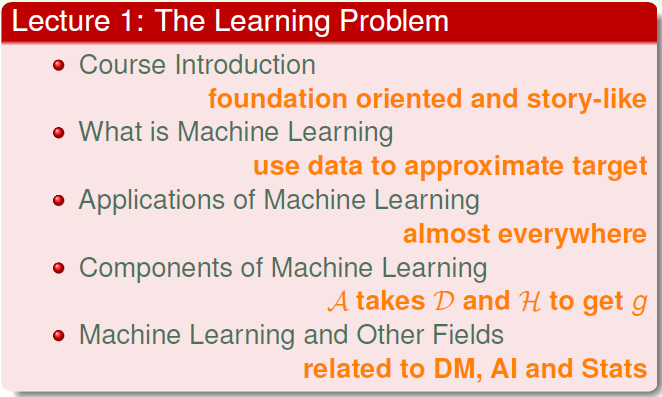
\includegraphics[width=10cm, height=6cm]{lecture1_sum}\\
\end{center}

\noindent
{\color{RubineRed} \rule{\linewidth}{1mm} }
% {\color{LightRubineRed} \rule{\linewidth}{1mm} }

%%%%%%%%%%%%%%%%%%%%%%%%%%%%%%%%%%%%%%%%%%%%%%%%%%%%%section 2
\section{Learning to Answer Yes/No} % (fold)
\noindent
{\color{LightRubineRed} \rule{\linewidth}{1mm} }
\subsection{Perceptron}
\begin{align*}
h(x) &= sign((\sum_{i=1} W_i x_i - \text{threshold})) \\
     &= sign((\sum_{i=0} W_i x_i)) \\
     &= sign(W^TX)
\end{align*}
\begin{center}
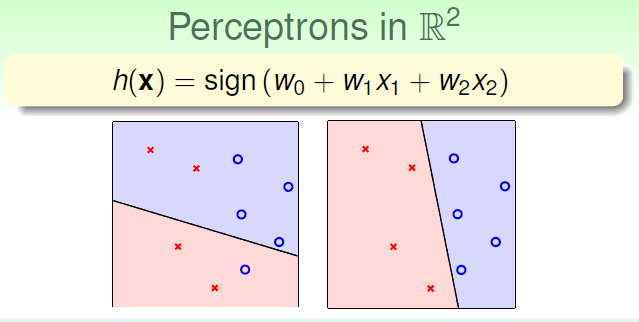
\includegraphics[width=10cm, height=5cm]{lecture2_1}\\
\end{center}
\begin{algorithm}  
\caption{Perceptron Learning Algorithm}  
\begin{algorithmic}  
\FOR{$t\gets1$ to $m$ }  
	\STATE Find a \textcolor{Mycolor1}{mistake} of $W_t$
	\STATE eg. $sign(W_{t}^{T}x_{n(t)}) \neq y_{n(t)}$ 
	\STATE $W_{t+1} \gets W_{t} + y_{n(t)}x_{n(t)}$ 
\ENDFOR
% \STATE return $W$(called W_{PLA})
\end{algorithmic}  
\end{algorithm}
缺点就是必须线性可分 Linear Separability \par
\begin{center}
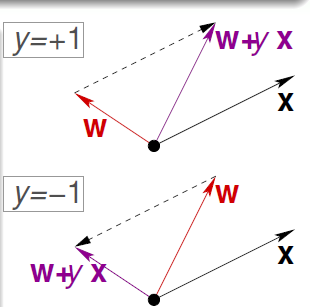
\includegraphics[width=5cm, height=5cm]{lecture2_2}\\
PLA \par
\end{center}
PLA Fact: $W_t$ Gets more Aligned with $W_f$,学习是能够保证$W$逐渐趋近于理想的$W_f$,
内积越大越相似。\par
\begin{align*}
w_f^{T}w_{t+1} &= w_f^{T}(w_t + y_{n(t)}x_{n(t)}) \\
               &\geq w_f^{T}w_t + \underset{n}{\min}y_nw_f^Tx_n \\
               &> w_f^Tw_t + 0.
\end{align*}
因此整个更新过程是$w_f \gets w_t$的,但有时候数据是有噪音的或者本身就不可分。 \par
% section section_name (end)
\begin{center}
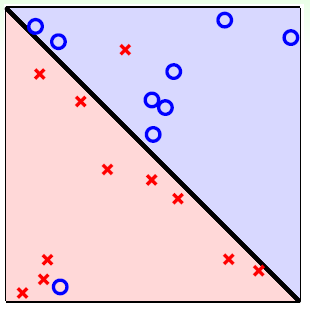
\includegraphics[width=5cm, height=5cm]{lecture2_3}\\
\end{center}
\subsection{Pocket}
\begin{algorithm}  
\caption{Pocket Algorithm}  
\begin{algorithmic}  
\STATE initialize pocket weights $\hat{w}$
\FOR{$t\gets1$ to $m$ }  
	\STATE 1.Find a \textcolor{Mycolor1}{mistake} of $W_t$
	\STATE eg. $sign(W_{t}^{T}x_{n(t)}) \neq y_{n(t)}$ 
	\STATE 2.$W_{t+1} \gets W_{t} + y_{n(t)}x_{n(t)}$ 
	\STATE 3.$W_{t+1} \gets \arg\underset{mistakes}{\min}(\hat{w},w_t)$
\ENDFOR
% \STATE return $W$(called W_{PLA})
\end{algorithmic}  
\end{algorithm}
\par
%%%%%%%%%%%%%%%%%%%%%Method one
\begin{bclogo}{Important!}
对PLA算法一个简单的修改(Pocket里永远是最好的),能处理有少许噪音的数据,但是速度要慢一点因为有比较的过程。 \par
\end{bclogo}
%%%%%%%%%%%%%%%%%%%%%Method tow
\begin{myremark}{Importance}
对PLA算法一个简单的修改(Pocket里永远是最好的),能处理有少许噪音的数据,但是速度要慢一点因为有比较的过程。 \par
\end{myremark}

\begin{center}
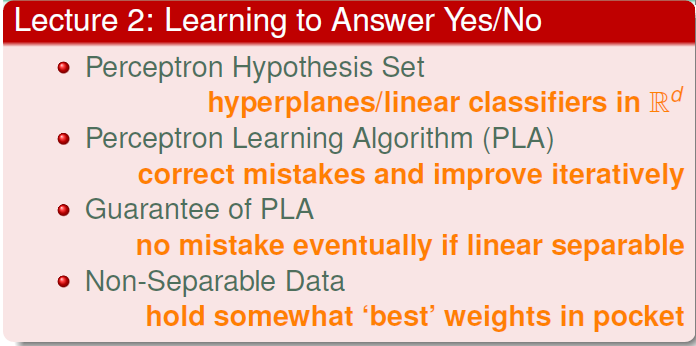
\includegraphics[width=10cm, height=5.5cm]{lecture2_sum}\\
\end{center}

\noindent
{\color{RubineRed} \rule{\linewidth}{1mm} }
\section{Types of Learning} % (fold)
\noindent
{\color{LightRubineRed} \rule{\linewidth}{1mm} }
\begin{itemize}
\item \textbf{Binary classification}:\par
patient features $\Rightarrow$ sick or not 
\begin{align}
\mathcal{Y} = \{-1,+1\}
\end{align}
\item \textbf{Multiclass Classification}: \par
pathent features $\Rightarrow$ which type of cancer 
\begin{align}
\mathcal{Y} = \{1,2,...,K\}
\end{align}
\item \textbf{regression}: \par
pathent features $\Rightarrow$ how many days before recoverry 
\begin{align}
\mathcal{Y} = \mathbb{R}
\end{align}
\item \textbf{Sequence Learning}: \par
NLP
\end{itemize}
\begin{center}
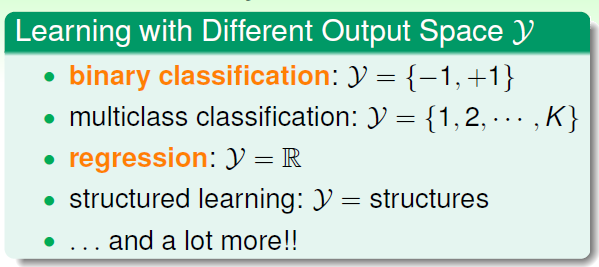
\includegraphics[width=10cm, height=5cm]{lecture3_1}\\
\end{center}
% section section_name (end)
\noindent
{\color{LightRubineRed} \rule{\linewidth}{1mm} }
\begin{itemize}
\item Supervised \par
\item Unsupervised \par
\item Semi-supervised \par
\item Reinforcement
\end{itemize}
\begin{center}
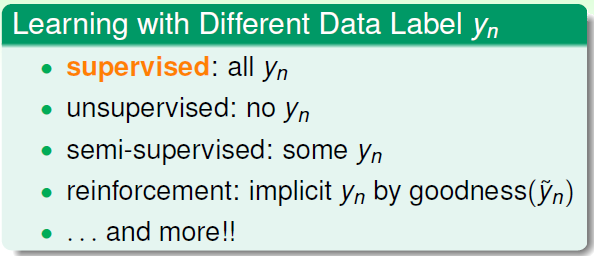
\includegraphics[width=10cm, height=4.5cm]{lecture3_2}\\
\end{center}
输入,输出,训练模式,算法类型。
\begin{center}
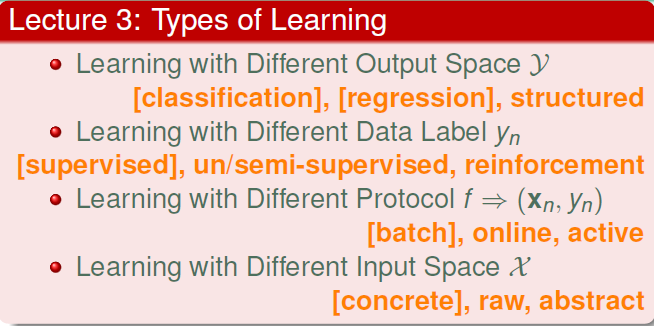
\includegraphics[width=10cm, height=5cm]{lecture3_sum}\\
\end{center}
\noindent
{\color{RubineRed} \rule{\linewidth}{1mm} } 
\section{Feasibility of Learning}
\noindent
{\color{LightRubineRed} \rule{\linewidth}{1mm} }

\subsection{No Free Lunch}
Learning from $D$ (to infer something outside$D$) is doomed if any 'unknown' $f$ can happen. :( \par

\subsection{Inferring something} % (fold)
\begin{center}
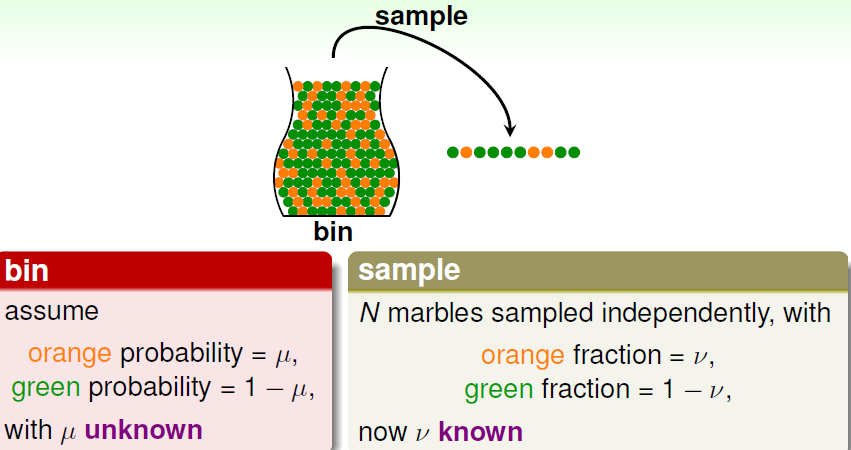
\includegraphics[width=10cm, height=6.5cm]{lecture4_1}\\
\end{center}
\textbf{Hoeffding's Inequality} \par
坏事情发生的几率有多大 \par
\begin{align*}
\mathbb{P}[|\nu-\mu| > \epsilon] \leq 2\exp(-2\epsilon^2N)
\end{align*}
跟$\mu$无关,跟$N$有关,如果样本够多,大概可以去近似。 \par
\subsection{Connection to Learning} % (fold)
\begin{align*}
E_{out}(h) &= \underset{x \sim P}{E} \llbracket h(x) \neq f(x) \rrbracket\\
E_{in}(h) &= \frac{1}{N}\sum_{n=1}^N \llbracket h(x) \neq f(x) \rrbracket \\
\end{align*}
$E_{in}$in-of-sampling(Known) \\
$E_{out}$out-of-sampling(UnKnown) \\
就像刚才一样我们不需要知道$E_{out}$,只需要$N$足够大即可。\par
\begin{align*}
\mathbb{P}[|E_{in}-E_{out}| > \epsilon] \leq 2\exp(-2\epsilon^2N)
\end{align*}
这样从理论保证,对于固定的$h$,如果数据足够多的话。
\begin{align*}
	E_{in} \approx E_{out}
\end{align*}
\subsection{Multiple h} % (fold)
Bound of Bad data \par
\begin{align*}
%http://ccxxxx.blog.51cto.com/7769075/1339606
\mathbb{P}_D[\text{bad} \ \mathcal{D}] \\
&= \mathbb{P}_D[\text{bad} \ \mathcal{D} \; for \; all \; h] \\
&\leq 2M\exp{-2\epsilon^2N}
\end{align*}
如果算法$A$找到一个$g$保证$E_{in} \approx 0$,那么理论保证$E_{out} \approx 0$ \\
$M$应该代表了复杂度,$N$代表了数据多少,理解这两个数值对ML的优化很有帮助。 
\begin{center}
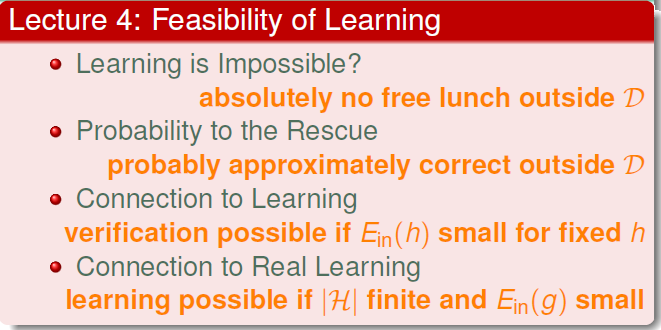
\includegraphics[width=10cm, height=6cm]{lecture4_sum}
\end{center}
\noindent
{\color{RubineRed} \rule{\linewidth}{1mm} }

\chapter{Why Can machines Learn?}
\section{Training versus Testing} % (fold)
\noindent
{\color{LightRubineRed} \rule{\linewidth}{1mm} }
\begin{bclogo}{Importance}
\begin{align*}
\mathbb{E}_{out}(g) \underbrace{\approx}_{\text{test}} \mathbb{E}_{in}(g) \underbrace{\approx}_{\text{train}} 0
\end{align*}
\end{bclogo}
\subsection{Effective Number lines} % (fold)
\label{sub:effective_number_lines}
\begin{center}
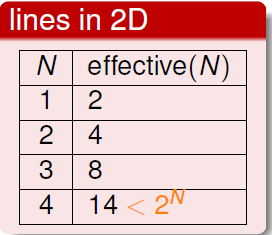
\includegraphics[width=6cm, height=6.5cm]{lecture5_2}\\
\end{center}
\begin{itemize}
	\item effective(N) can replace $M$ and
	\item effective(N) << $2^N$
\end{itemize}
\subsection{Effective Number of Hypotheses}
dichotomies 二分 \par
\begin{center}
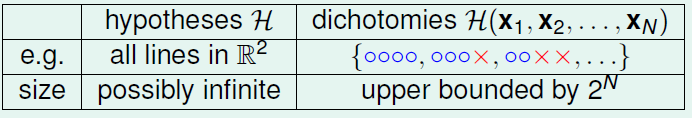
\includegraphics[width=10cm, height=4cm]{lecture5_1}\\
\end{center}
\begin{align*}
m_{\mathcal{H}}(N)=2^N \rightleftharpoons 
\end{align*}
text{exists} $N$ \text{inputs that can be shattered}

\subsection{Break Point}
if no $K$ inputs can be shatted by $H$, \par
call k a break point for $H$。
\begin{align}
m_{\mathcal{H}}(k) < 2^K \\
k+1,k+2,.. \text{also break points} \\
\end{align}
break points跟成长函数是有关的 。 \\

\begin{center}
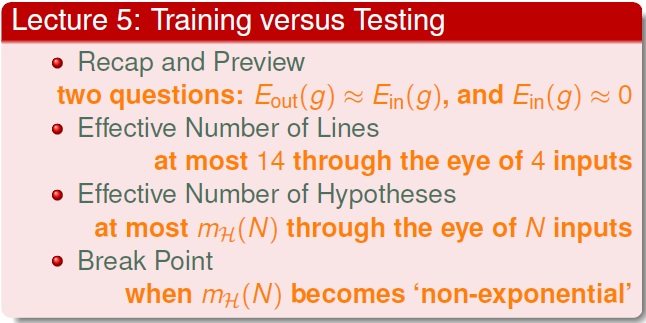
\includegraphics[width=10cm, height=6cm]{lecture5_sum}\\
\end{center}
% subsubsection effective_number_lines (end)
% section section_name (end)
\noindent
{\color{RubineRed} \rule{\linewidth}{1mm} }
\section{Theory of Generalization}
\noindent
{\color{RubineRed} \rule{\linewidth}{1mm} }

Theory of Generalization. \par
\noindent
{\color{LightRubineRed} \rule{\linewidth}{1mm} }
\section{VC demension}
\noindent
{\color{RubineRed} \rule{\linewidth}{1mm} }

\subsection{Definition of VC Dimension} % (fold)
\label{sub:definition_of_vc_dimension}
视频不想看了。 
%http://www.flickering.cn/machine_learning/2015/04/vc%E7%BB%B4%E7%9A%84%E6%9D%A5%E9%BE%99%E5%8E%BB%E8%84%89/
% subsection definition_of_vc_dimension (end)VC demension
\noindent
{\color{LightRubineRed} \rule{\linewidth}{1mm} }
\section{Noise and Error}
\noindent
{\color{RubineRed} \rule{\linewidth}{1mm} }
Target Distributiion but not Target Function \par
\textbf{VC} still works. \par

\subsection{Error Measure}
用来判别$f$是否有效。 \par
\textbf{0/1 error}
\begin{align*}
E(\hat{y},y) = \llbracket \hat{y} \neq y \rrbracket
\end{align*}
\textbf{squared error}
\begin{align*}
E(\hat{y},y) = (\hat{y} -y)^2
\end{align*}
不同的error 'Guide' Learning 效果也不同。 \par
\subsection{Weighted Classification}
CIA cost vs. market cost \par
Copy一些样本就相当于在这些样本上增加了weight。 \par\par
\begin{center}
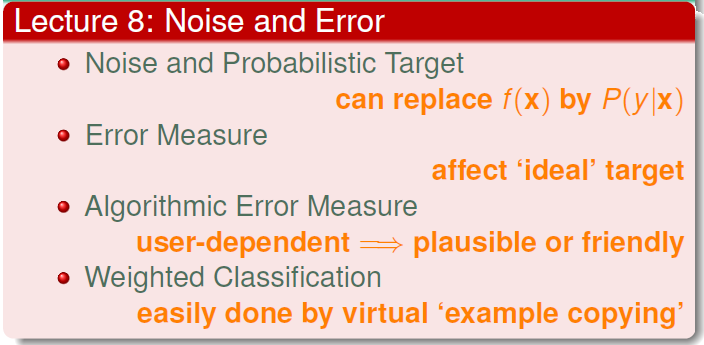
\includegraphics[width=10cm, height=5cm]{lecture8_sum}\\
\end{center}
\noindent
{\color{LightRubineRed} \rule{\linewidth}{1mm} }
\chapter{How Can machines Learn?}
\section{Linear Regression}
\noindent
{\color{LightRubineRed} \rule{\linewidth}{1mm} }
\subsection{Linear Regression hypothesis}
\begin{align*}
h(x) = W^Tx
\end{align*}
\begin{myremark}{Importance}
Find \textcolor{mypink2}{lines/hyperplanes} with small \textcolor{mypink3}{residuals}.
\end{myremark}
\textbf{The Error Measure}
\begin{align*}
E_{in}(w) &= \frac{1}{N}\sum_{n=1}^N  (w^Tx_n - y_n)^2 \\
E_{out}(h) &= \underset{x \sim P}{\mathbb{E}} (w^Tx_n - y_n)^2\\
\end{align*}
\textbf{Min $E_{in}$ ?} 
\subsection{Linear Regression Algorithm}
\begin{align*}
E_{in}(w) &= \frac{1}{N}\sum_{n=1}^N  (w^Tx_n - y_n)^2 \\
          &= \frac{1}{N} {||XW -Y||}^2
\end{align*}
\begin{align*}
\; let \ \nabla_{w}E = 0 \\
E_{in}(W) &= \frac{1}{N} {||XW -Y||}^2 \\
       &= \frac{1}{N} (W^T\underbrace{X^TX}_AW - W^T\underbrace{X^Ty}_b + \underbrace{y^Ty}_c) \\
       &= \frac{1}{N}(W^TAW - 2W^Tb + c) \\
\nabla_{W}E &= \frac{1}{N}(2AW-2b) \\
            &= \frac{2}{N}(AW-b) \\
            &= 0 \\
W^* = \underbrace{(X^TX)^{-1}X^T}_{pseudo-inverse}y
\end{align*}
\subsection{Generalization issue}
不像是一个学习的过程,而是一步登天。 \par
不是特别懂呀。。 \par

\subsection{Linear Classification vs. Linear Regression}
\begin{center}
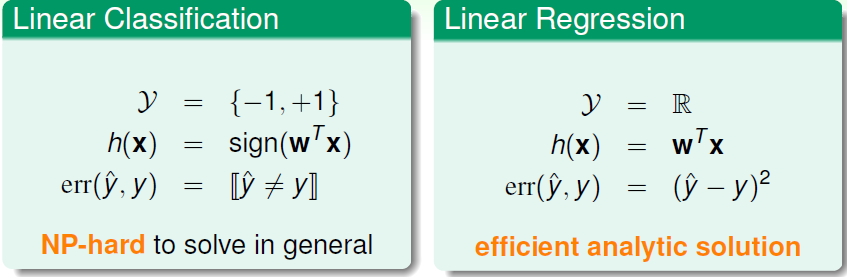
\includegraphics[width=10cm, height=4cm]{lecture9_1}\\
\end{center}
可以用LR来优化linear Classification。VC 理论可以保证学习。 \par
\begin{center}
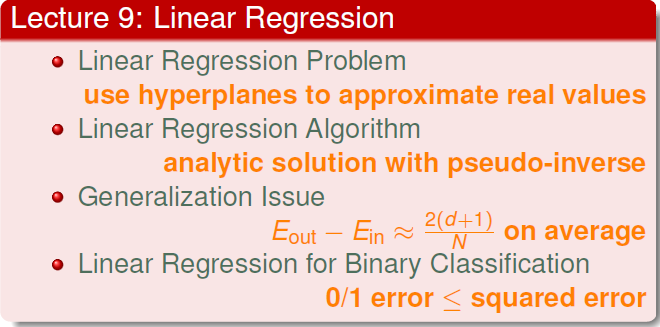
\includegraphics[width=8cm, height=5cm]{lecture9_sum}\\
\end{center}

\noindent
{\color{RubineRed} \rule{\linewidth}{1mm} }
\section{Logistic Regression}
\noindent
{\color{LightRubineRed} \rule{\linewidth}{1mm} }

\subsection{Logistic Regression Problem} % (fold)
\label{sub:logistic_regression_problem}
% better than align* ?
\begin{gather*}
f(x) = \mathcal{P}(+1 | x ) \in [0,1]
\end{gather*}
% subsection logistic_regression_problem (end)
\subsection{Logistic Hypothesis} % (fold)
\label{sub:logistic_hypothesis}
\begin{align*}
h(x) &= \theta{(W^TX)} \\
     &= \frac{1}{1+\exp{(-W^TX)}} \\
\theta(s) &= \frac{1}{1+\exp{(-s)}}
\end{align*}
\textbf{Sigmoid}: smooth,monotonic \par
% subsection logistic_hypothesis (end)
\subsection{Three Linear Models}
\textbf{linear scoring function}: \par
\begin{gather*}
S = W^TX
\end{gather*}
\begin{center}
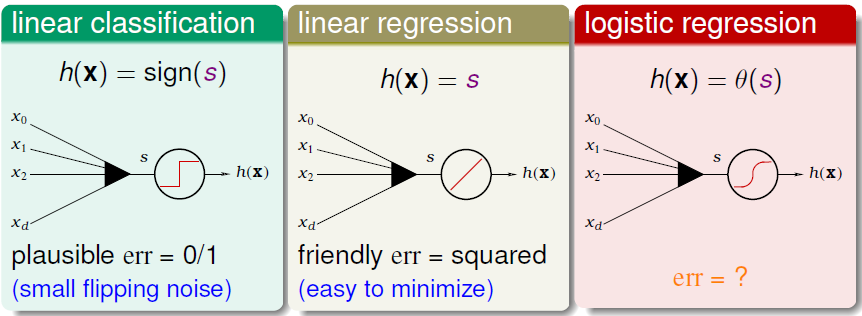
\includegraphics[width=14cm, height=5cm]{lecture10_1}\\
\end{center}
\textbf{Likelihood}
\begin{gather*}
\mathcal{P}(y|x) = 
\left\{  
             \begin{array}{lr}  
             f(x), &for \ y = + 1  \\  
             1- f(x), &for \ y= -1    
             \end{array}  
\right.  
\end{gather*}
\begin{align*}
 g^* &= \arg \underset{h}{max}\ \text{likelihood}(h) \\
 g^* & \propto \prod_{n=1}h(y_nx_n)
\end{align*}
\textbf{Cross-Entropy}
\begin{align*}
 \text{likelihood}{(w)} &\propto \underset{w}{\max} \prod \theta{(y_nW^Tx_n)} \\
 &\propto \underset{w}{\max} \log\prod\theta{(y_nW^Tx_n)} \\
 &\propto \underset{w}{\min} \sum - \log\theta{(y_nW^Tx_n)} \\
 &\propto \underset{w}{\min} \sum \log(1+\exp(-y_nW^Tx_n)) \\
 &\propto \underset{w}{\min} \sum \text{err}(W,x_n,y_n) \\
\end{align*}
 
\subsection{Minimizing $E_{in}(W)$}
用梯度链法求梯度就行了。 \par
求完梯度不像LR一样是close-form,一步登天。 \par
借鉴PLA思想iterative Optimization \par
\begin{align*}
w_{t+1} \gets w_t + \underbrace{1}_\eta \underbrace{\llbracket sign(w^Tx) \neq y_n\rrbracket * y_nx_n }_{\nu}
\end{align*}

\subsection{Gradient Descent}
尽管不能一次算出最好的$E_{in}$,可以用Greedy approch \par
\begin{align*}
W_{t+1} \gets W_t + \eta V \\
\underset{||v||=1}{\min} E_{in}(\underbrace{W_t+ \eta V}_{W_{t+1}})
\end{align*}
对于比较小的 $\eta$可以使用泰勒展开 
\begin{align*}
E_{in}(W_t+\eta V) \approx E_{in}(W_t) + \eta v^T \nabla E_{in}(W_t)
\end{align*}
要使$E_{in}(W_{t+1})$ 最小化,我们只需要保证$V$的方向和$\nabla$的\textcolor{mypink2}{方向相反}并且大小相同即可。(V即是W要走的方向)
\begin{align*}
V = -\frac{\nabla}{||\nabla||}
\end{align*}
\begin{myremark}{SGD}
\begin{align*}
W_{t+1} \gets W_t - \eta \frac{\nabla}{||\nabla||}  \\
\end{align*}
\end{myremark}
不同的$\eta$影响效果也不同,一个启发式的做法是根据梯度的模重新定义$\eta$ \par
\begin{center}
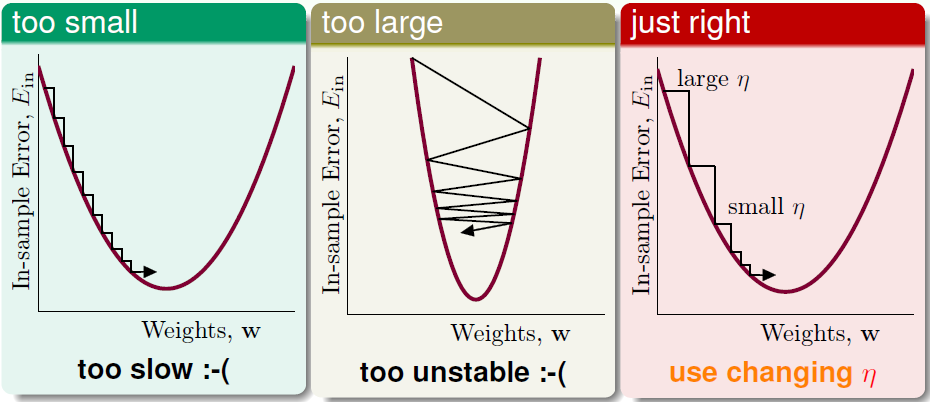
\includegraphics[width=14cm, height=5cm]{lecture10_2}\\
\end{center}
其实就是GD,算法不写了。
\begin{center}
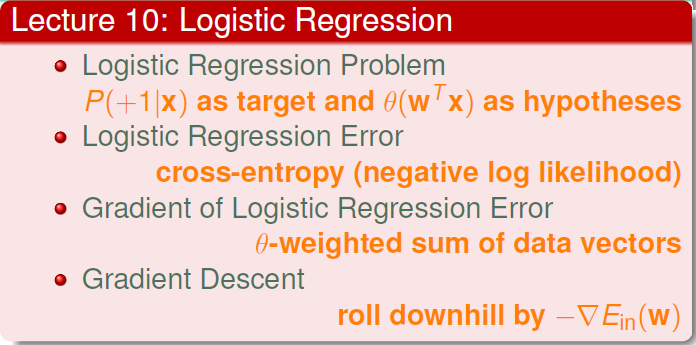
\includegraphics[width=10cm, height=5.5cm]{lecture10_sum}\\
\end{center}
\noindent
{\color{RubineRed} \rule{\linewidth}{1mm} }
\section{Linear Models for Classification}
\noindent
{\color{LightRubineRed} \rule{\linewidth}{1mm} }
%%%%%%%%%%%%%%
\subsection{Linear Models Revisited}
\begin{center}
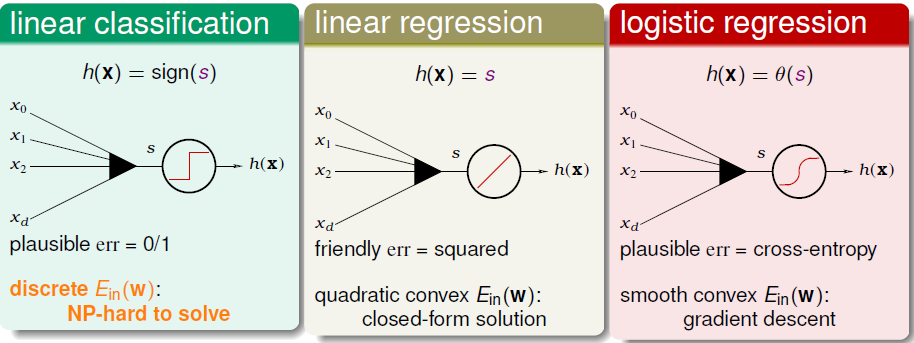
\includegraphics[width=14cm, height=5cm]{lecture11_1}\\
\end{center}
\textbf{Error Functions Revisited} \par
(ys)表示了一定的物理意义。 
\begin{center}
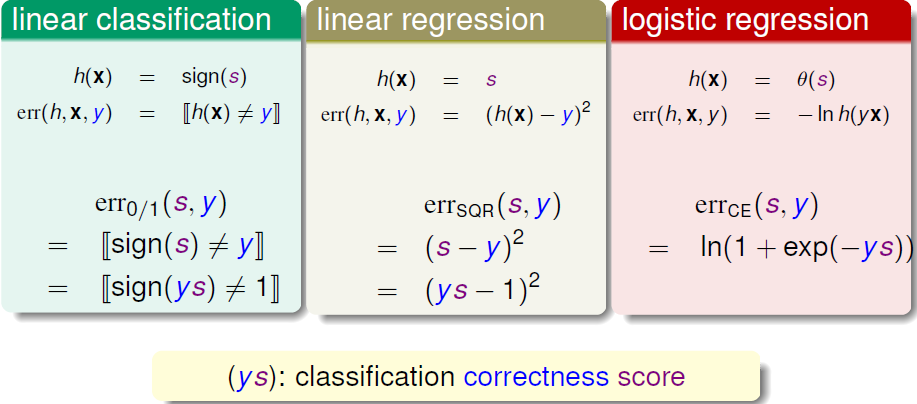
\includegraphics[width=14cm, height=6cm]{lecture11_2}\\
\end{center}
\begin{center}
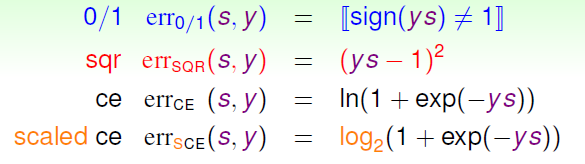
\includegraphics[width=10cm, height=3.5cm]{lecture11_3}\\
\end{center}
\begin{center}
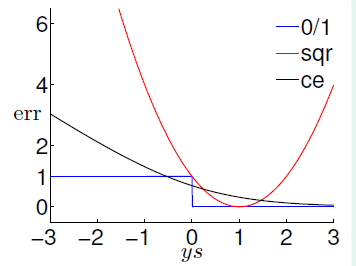
\includegraphics[width=8cm, height=6cm]{lecture11_4}\\
\end{center}
%%%%%%%%%%%%%%%%
\subsection{Stochastic Gradient Decent}
\begin{align*}
w_{t+1} \gets w_t + \eta \frac{1}{N}\sum_{n=1}\nabla_i
\end{align*}
N的数据量实在太大,我们可以使用随机抽样的方式进行。SGD = GD + zero-mean 'noise' 。用随机梯度代替真实梯度,迭代足够step后,平均随机梯度趋近于平均真是梯度。这样做简单,计算量小,适合大数据,online learning,SGD全靠抖,不是特别稳定比较GD而言。 \par

\begin{align*}
w_{t+1} \gets w_t + \eta\nabla_i
\end{align*}
SGD算法很像PLA \par
\begin{center}
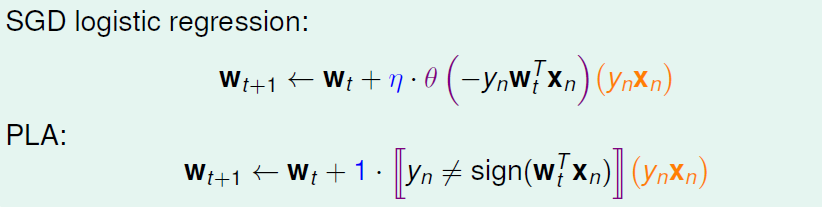
\includegraphics[width=8cm, height=2.5cm]{lecture11_5}\\
\end{center}

\subsection{Multiclass via Binary}
\begin{itemize}
	\item One vs. All [One class at a Time]
	\item One vs. One []
\end{itemize}
\begin{center}
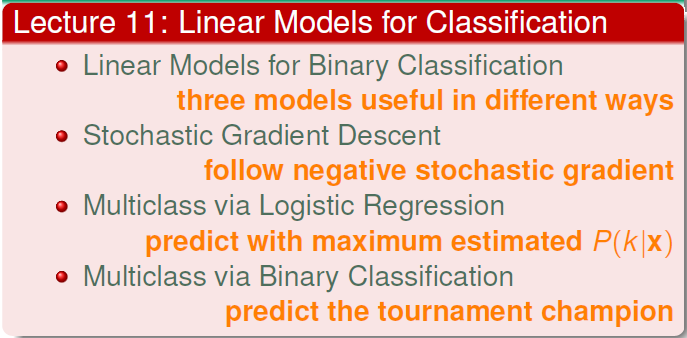
\includegraphics[width=10cm, height=5cm]{lecture11_sum}\\
\end{center}
\noindent
{\color{RubineRed} \rule{\linewidth}{1mm} }

\section{Nonlinear Transformation}
\noindent
{\color{LightRubineRed} \rule{\linewidth}{1mm} }
%%%%%%%%%%%%%%
\begin{align*}
x \in \mathcal{X} \overset{\Phi}{\rightarrow} \ z \in \mathcal{Z}
\end{align*}
perceptrons in $Z$-space = quadratic hypotheses in $X$-space \par
%%%%%%%%%%%%%%
Linear/simpler model first. \par
\begin{center}
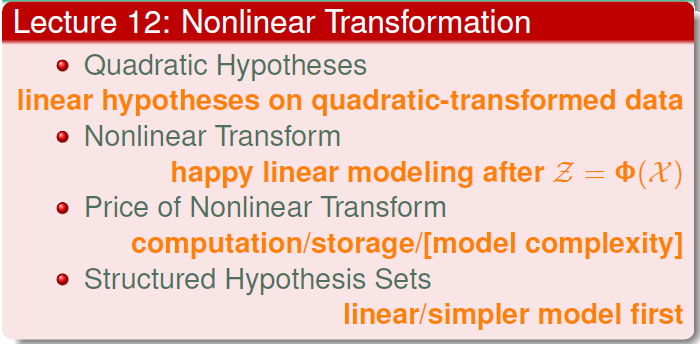
\includegraphics[width=10cm, height=5cm]{lecture12_sum}\\
\end{center}
\noindent
{\color{RubineRed} \rule{\linewidth}{1mm} }
\chapter{How Can machines Learn Better?}
\section{Hazard of Overfitting}
\noindent
{\color{LightRubineRed} \rule{\linewidth}{1mm} }
\subsection{What is Overfitting} % (fold)
\label{sub:what_is_overfitting}
\textcolor{mypink2}{Hazard} : 冒险 \par
\textbf{Bad Generalizaton} \par
low $E_{in}$,high $E_{out}$. \par
\begin{myremark}{}
不管模型多复杂$M$,或者数据量多少$N$,其实就以下两个考虑。 \par
\begin{align*}
\mathbb{E}_{out} \approx \mathbb{E}_{in} \approx 0 \\
\end{align*}
即使$E+{in}$非常小有什么用?作为预测使用我们需要的是$E_{out}$。
\end{myremark}
下图揭示了模型大小,与数据量大小的关系。 \par
\begin{center}
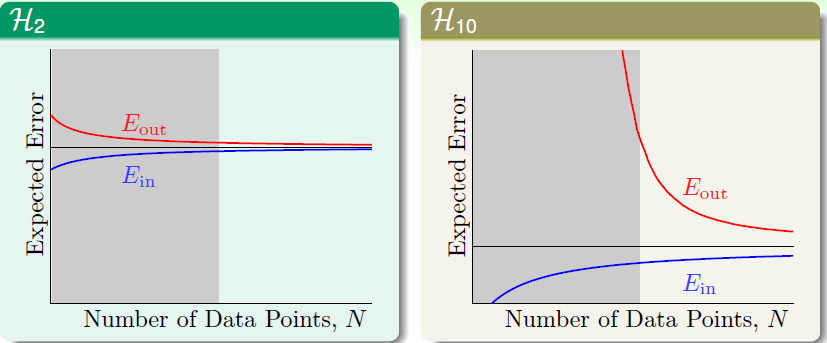
\includegraphics[width=10cm, height=5cm]{lecture13_1}\\
\end{center}
% subsection what_is_overfitting (end)

\subsection{Dealing with Overfitting} % (fold)
\label{sub:dealing_with_overfitting}
\begin{center}
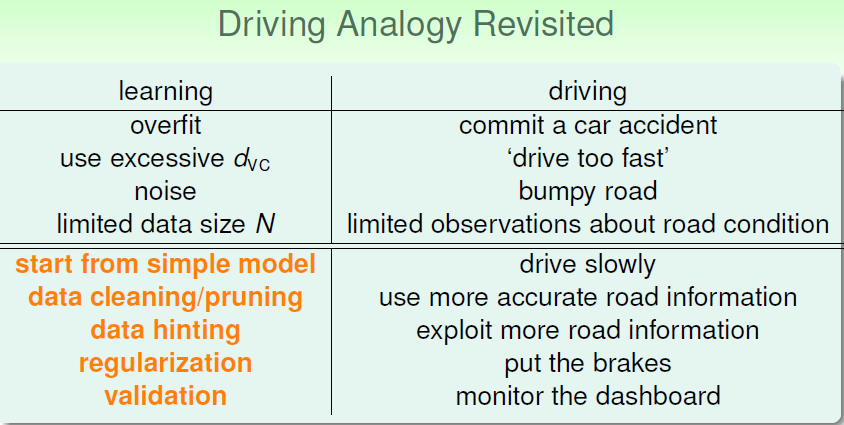
\includegraphics[width=10cm, height=6cm]{lecture13_2}\\
\end{center}
% subsection dealing_with_overfitting (end)
\begin{center}
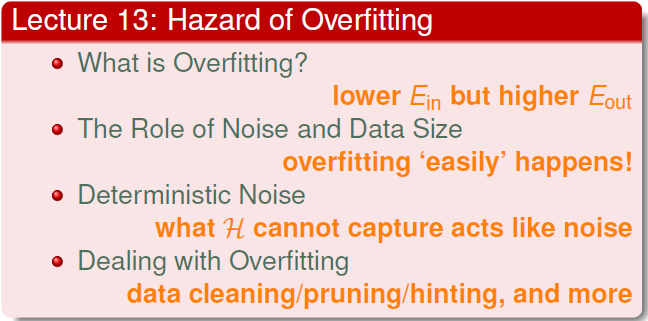
\includegraphics[width=10cm, height=5cm]{lecture13_sum}\\
\end{center}
\noindent
{\color{RubineRed} \rule{\linewidth}{1mm} }
\section{Regularization}
\noindent
{\color{LightRubineRed} \rule{\linewidth}{1mm} }
%%%%%%%%%%%%%%
\subsection{Regularized Hypothesis Set} % (fold)
\label{sub:regularized_hypothesis_set}
模型复杂度大,不是容易overfitting么,那么限制一下权值大小(多少)。 \par
\begin{center}
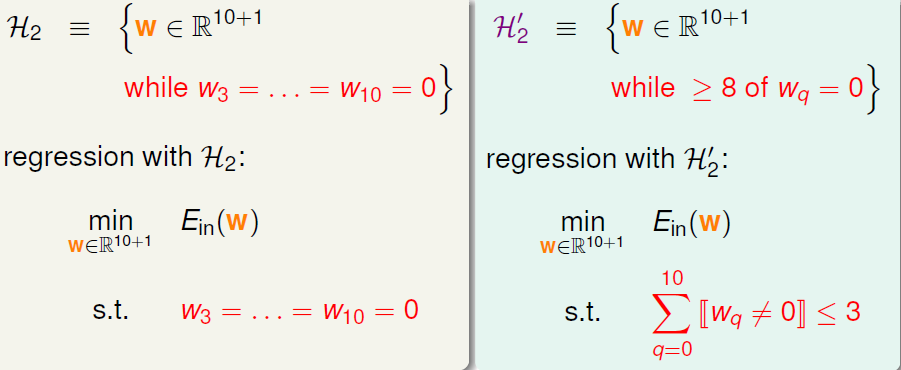
\includegraphics[width=12cm, height=4cm]{lecture14_1}\\
\end{center}
直接限制$W$个数,优化是$NP$,bad news for \textcolor{mypink3}{sparse hypothesis Set}.因此可以Softer下。
\begin{center}
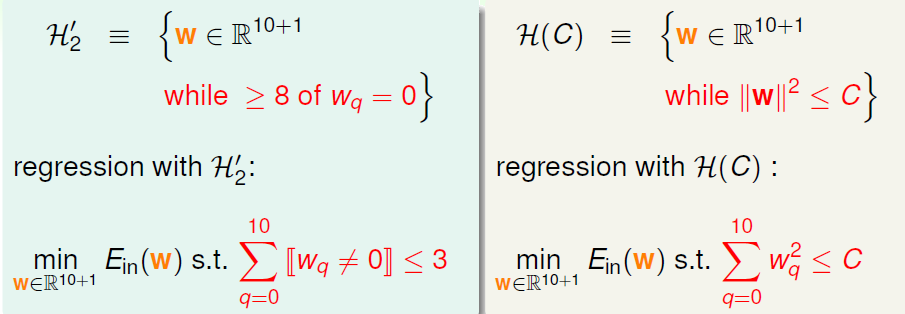
\includegraphics[width=12cm, height=4cm]{lecture14_2}\\
\end{center}

\subsection{Weight Decay Regularization} % (fold)
这样的意思就是把$W$现在在一个$\sqrt{C}$的圆里边。
\begin{align*}
\underset{w \in \mathbb{R}^{Q+1}}{\min} \ &E_{in}(w) = \frac{1}{N}\sum_{n=1}(w^Tz-y)^2 \\
s.t. \quad &\underbrace{\sum_{q=0}w_q^2}_{w^Tw} \leq C
\end{align*}
负的梯度方向可以垂直分解为圆的切线和法线方向。但是$C$限制了法线方向因此只能沿着圆的切线方向移动。因此$W_{reg}$的最优解是:负的梯度方向和法线方向是平行的。 \par
\begin{center}
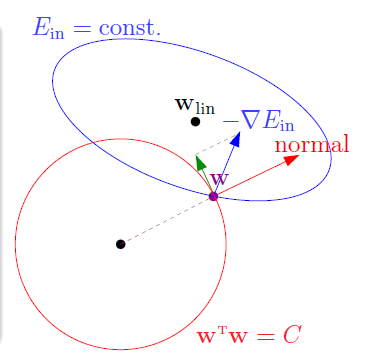
\includegraphics[width=5cm, height=5cm]{lecture14_3}\\
\end{center}
\begin{align*}
-\nabla{E_{in}{W_{reg}}} \propto W_{reg}
\end{align*}
使用有条件最优化工具Lagrange multiplier,可以模仿线性回归解正规方程了,也叫ridge regression。另外可以根据梯度公式推导出新的优化公式,这也是常见的L2正规化公式。\par
\begin{align*}
&\nabla{E_{in}(W) + \frac{2\lambda}{N}W} = 0 \\
&W \gets (Z^TZ + \lambda I)^{-1}Z^Ty \\
\end{align*}
\begin{align*}
solve \ \ &\nabla{E_{in}(W) + \frac{2\lambda}{N}W} = 0 \\
\underset{W}{\min} \quad &E_{in}(W) + \frac{\lambda}{N}\overbrace{W^TW}^{regular}
\end{align*}


\subsection{Regularization and VC Theory} % (fold)
\label{sub:regularization_and_vc_theory}

% subsection regularization_and_vc_theory (end)
\subsection{General Regularizers} % (fold)
\label{sub:general_regularizers}
\textbf{\textcolor{mypink2}{L2 and L1}}
\begin{center}
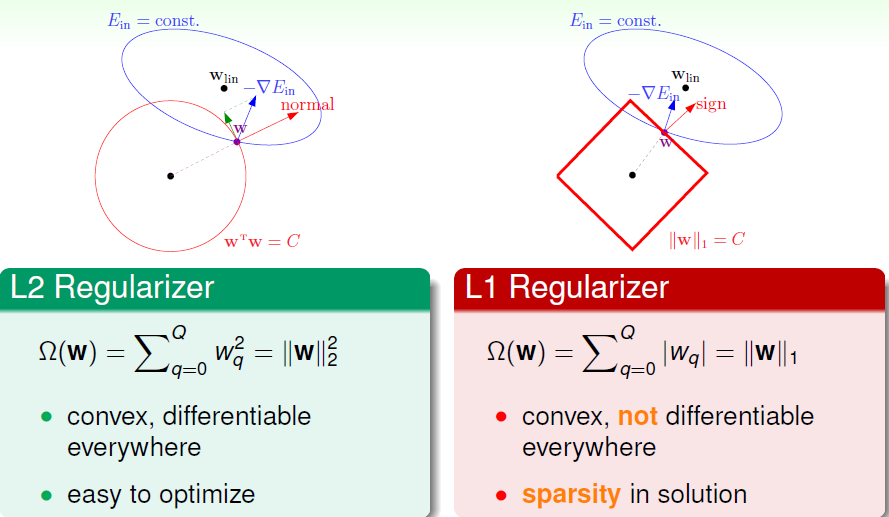
\includegraphics[width=10cm, height=7cm]{lecture14_4}\\
\end{center}
% subsection general_regularizers (end)
%%%%%%%%%%%%%%
\begin{center}
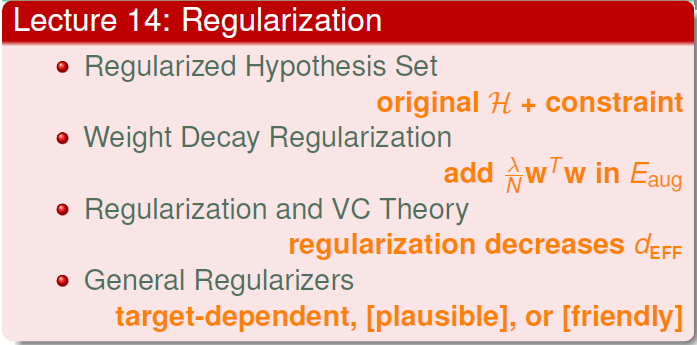
\includegraphics[width=10cm, height=5cm]{lecture14_sum}\\
\end{center}
\noindent
{\color{RubineRed} \rule{\linewidth}{1mm} }
\section{Validation}
\noindent
{\color{LightRubineRed} \rule{\linewidth}{1mm} }
%%%%%%%%%%%%%%
\subsection{Model Selection Problem} % (fold)
\label{sub:model_selection_problem}
\begin{align*}
E_{out} \approx E_{in} \approx 0
\end{align*}
selecting by $E_{in}$ is dangerous,因为模型在训练集训练过了,会overfitting \par
Model selection by Best $E_{test}$,但是测试集一般是看不到的,因此可以split出验证集。\par
% subsection model_selection_problem (end)

\subsection{Validation Set} % (fold)
\label{sub:validation_set}
$E_{val}$用于选择模型,桥接$E_{in}$和$E_{out}$.如果能保证$D_{val}$,$D_{train}$以及$D_{test}$都是iid的来自于同一个分布$P$的话,效果是有保证的。 \par
\begin{center}
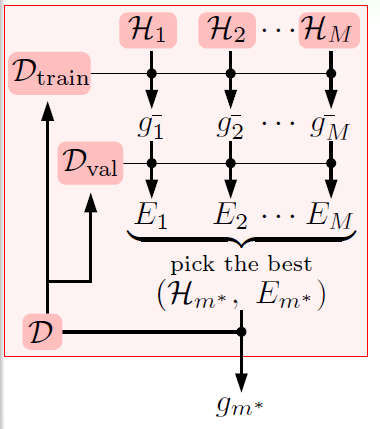
\includegraphics[width=4.5cm, height=6cm]{lecture15_1}
\end{center}
% subsection validation_set (end)

\subsection{Leave-One-Out Cross Validation} % (fold)
\label{sub:leave_one_out_cross_validation}

% subsection leave_one_out_cross_validation (end)
\subsection{V-fold Cross validation} % (fold)
\label{sub:v_fold_cross_validation}
交叉验证。
% subsection v_fold_cross_validation (end)
%%%%%%%%%%%%%%
\begin{center}
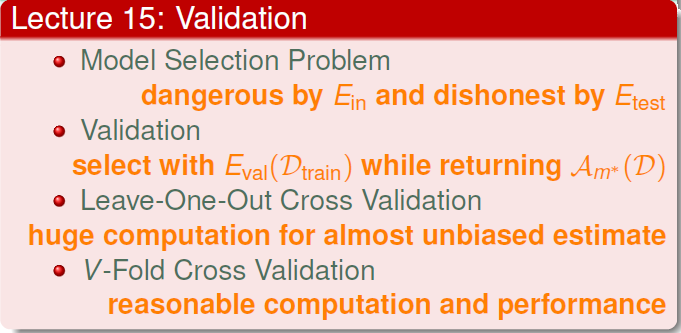
\includegraphics[width=10cm, height=5cm]{lecture15_sum}
\end{center}
\noindent
{\color{RubineRed} \rule{\linewidth}{1mm} }
\section{Three Learning Principles}
\noindent
{\color{LightRubineRed} \rule{\linewidth}{1mm} }
%%%%%%%%%%%%%%
\subsection{Occam's Razor} % (fold)
\label{sub:occam_s_razor}
\begin{myremark}{}
\Large{Simple is Better !!}
\end{myremark}
The simplest model that fits the data is also the most plausible. \par
% subsection occam_s_razor (end)

\subsection{Sampling Bias} % (fold)
\label{sub:sampling_bias}
\begin{myremark}{}
\Large{iid is importance !!}
\end{myremark}
If the data is sampled in biased way,learning will produce a similarly biased outcome. \par
\textcolor{mypink2}{\Large{Match test scenario(distribution)}} as much as possible.
% subsection sampling_bias (end)

\subsection{Data Snooping} % (fold)
\label{sub:data_snooping}
偷看数据很严重。 \par
\begin{center}
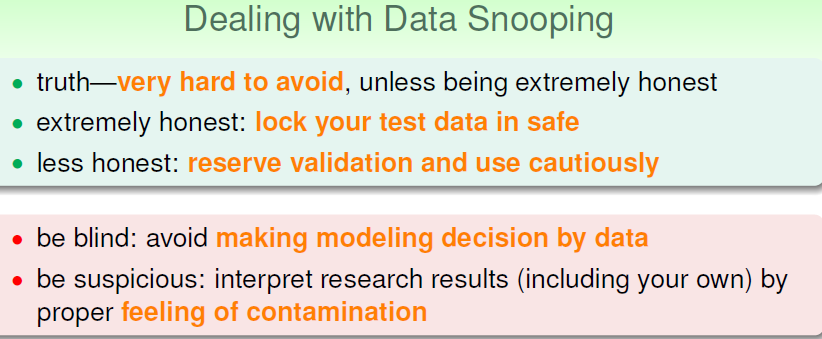
\includegraphics[width=10cm, height=4cm]{lecture16_1}
\end{center}
% subsection data_snooping (end)

\subsection{Three Related Fields} % (fold)
\label{sub:three_related_fields}
\begin{center}
\Large{Three Related Fields} \par
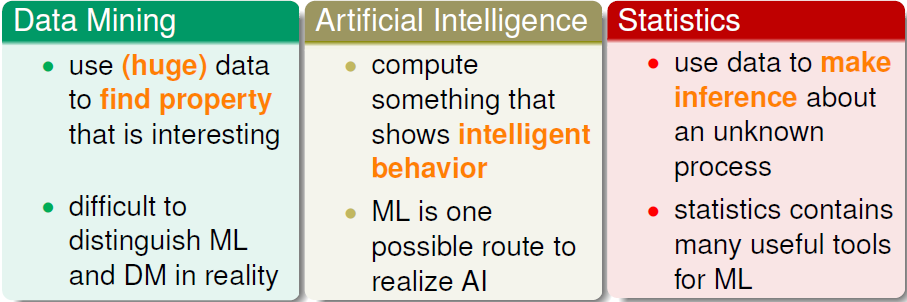
\includegraphics[width=14cm, height=5cm]{lecture16_2}
\end{center}

\begin{center}
\Large{Three Theoretical Bounds} \par
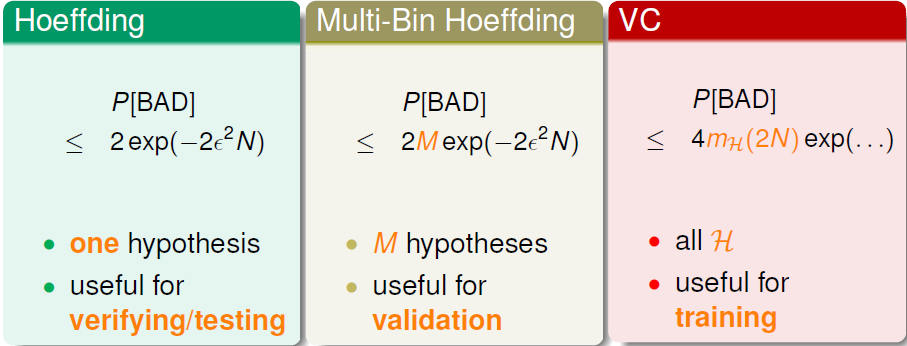
\includegraphics[width=14cm, height=5cm]{lecture16_3}
\end{center}

\begin{center}
\Large{Three Linear Models} \par
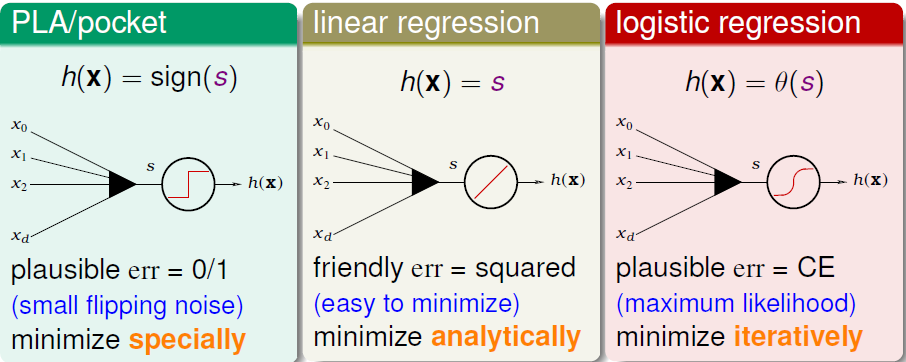
\includegraphics[width=14cm, height=5cm]{lecture16_4}
\end{center}

\begin{center}
\Large{Three Key Tools} \par
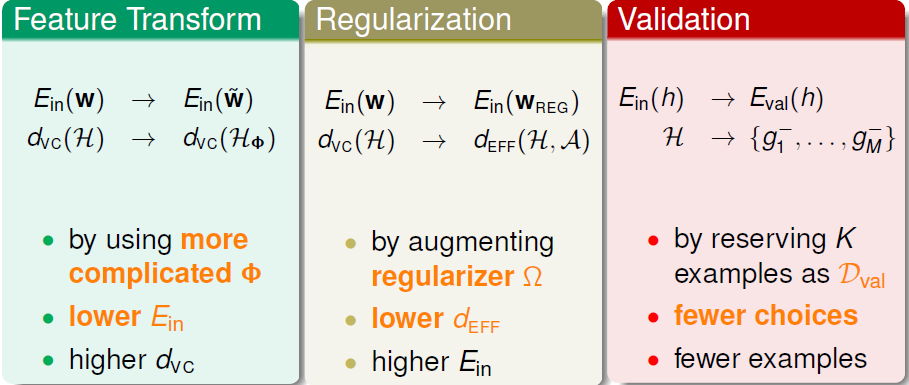
\includegraphics[width=14cm, height=5cm]{lecture16_5}
\end{center}

\begin{center}
\Large{Three Learning Principles} \par
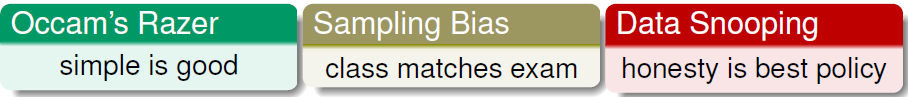
\includegraphics[width=14cm, height=2cm]{lecture16_6}
\end{center}
% subsection three_related_fields (end)
%%%%%%%%%%%%%%
\begin{center}
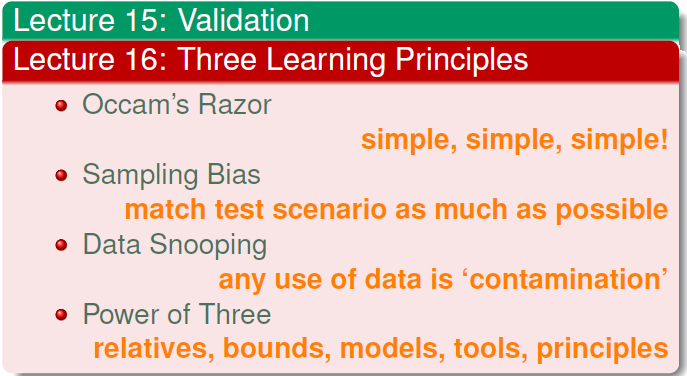
\includegraphics[width=14cm, height=5cm]{lecture16_sum}
\end{center}
\noindent
{\color{RubineRed} \rule{\linewidth}{1mm} }


\appendix
\chapter{附录}
没有附录。
\backmatter
\chapter{后记}
后记是什么的存在呢?

% \noindent
% {\color{LightRubineRed} \rule{\linewidth}{1mm} }
\end{document}